\documentclass[]{article}
\usepackage{lmodern}
\usepackage{amssymb,amsmath}
\usepackage{ifxetex,ifluatex}
\usepackage{fixltx2e} % provides \textsubscript
\ifnum 0\ifxetex 1\fi\ifluatex 1\fi=0 % if pdftex
  \usepackage[T1]{fontenc}
  \usepackage[utf8]{inputenc}
\else % if luatex or xelatex
  \ifxetex
    \usepackage{mathspec}
  \else
    \usepackage{fontspec}
  \fi
  \defaultfontfeatures{Ligatures=TeX,Scale=MatchLowercase}
\fi
% use upquote if available, for straight quotes in verbatim environments
\IfFileExists{upquote.sty}{\usepackage{upquote}}{}
% use microtype if available
\IfFileExists{microtype.sty}{%
\usepackage{microtype}
\UseMicrotypeSet[protrusion]{basicmath} % disable protrusion for tt fonts
}{}
\usepackage[margin=1in]{geometry}
\usepackage{hyperref}
\hypersetup{unicode=true,
            pdftitle={Rapport du projet},
            pdfauthor={Aimé Cazeel, Khadidiatou AW, Kokou Sossou},
            pdfborder={0 0 0},
            breaklinks=true}
\urlstyle{same}  % don't use monospace font for urls
\usepackage{graphicx,grffile}
\makeatletter
\def\maxwidth{\ifdim\Gin@nat@width>\linewidth\linewidth\else\Gin@nat@width\fi}
\def\maxheight{\ifdim\Gin@nat@height>\textheight\textheight\else\Gin@nat@height\fi}
\makeatother
% Scale images if necessary, so that they will not overflow the page
% margins by default, and it is still possible to overwrite the defaults
% using explicit options in \includegraphics[width, height, ...]{}
\setkeys{Gin}{width=\maxwidth,height=\maxheight,keepaspectratio}
\IfFileExists{parskip.sty}{%
\usepackage{parskip}
}{% else
\setlength{\parindent}{0pt}
\setlength{\parskip}{6pt plus 2pt minus 1pt}
}
\setlength{\emergencystretch}{3em}  % prevent overfull lines
\providecommand{\tightlist}{%
  \setlength{\itemsep}{0pt}\setlength{\parskip}{0pt}}
\setcounter{secnumdepth}{5}
% Redefines (sub)paragraphs to behave more like sections
\ifx\paragraph\undefined\else
\let\oldparagraph\paragraph
\renewcommand{\paragraph}[1]{\oldparagraph{#1}\mbox{}}
\fi
\ifx\subparagraph\undefined\else
\let\oldsubparagraph\subparagraph
\renewcommand{\subparagraph}[1]{\oldsubparagraph{#1}\mbox{}}
\fi

%%% Use protect on footnotes to avoid problems with footnotes in titles
\let\rmarkdownfootnote\footnote%
\def\footnote{\protect\rmarkdownfootnote}

%%% Change title format to be more compact
\usepackage{titling}

% Create subtitle command for use in maketitle
\providecommand{\subtitle}[1]{
  \posttitle{
    \begin{center}\large#1\end{center}
    }
}

\setlength{\droptitle}{-2em}

  \title{Rapport du projet}
    \pretitle{\vspace{\droptitle}\centering\huge}
  \posttitle{\par}
    \author{Aimé Cazeel, Khadidiatou AW, Kokou Sossou}
    \preauthor{\centering\large\emph}
  \postauthor{\par}
      \predate{\centering\large\emph}
  \postdate{\par}
    \date{3 février 2020}

\usepackage{booktabs}
\usepackage{longtable}
\usepackage{array}
\usepackage{multirow}
\usepackage{wrapfig}
\usepackage{float}
\usepackage{colortbl}
\usepackage{pdflscape}
\usepackage{tabu}
\usepackage{threeparttable}
\usepackage{threeparttablex}
\usepackage[normalem]{ulem}
\usepackage{makecell}
\usepackage{xcolor}

\begin{document}
\maketitle

{
\setcounter{tocdepth}{2}
\tableofcontents
}
\newpage

\hypertarget{ruxe9sumuxe9}{%
\section{Résumé}\label{ruxe9sumuxe9}}

Le CBSM ou Cognitive Behavioral Stress Management est un programme de
gestion du stress qui mélange des exercices de relaxation, de
restructuration cognitive et de dynamique de groupe.Si ce programme
étudié principalement aux Etats-Unis s'avère efficace sur des maladies
comme le cancer du sein ou le VIH, il n'existe cependant que peu
d'études sur l'application du programme CBSM sur des patients atteints
de maladies cardio-vasculaires et de son effet sur le stress, l'anxiété
et les pensées intrusives.

Ainsi, l'objectif de ce document est d'étudier l'efficacité de ce
programme auprès de patients atteints de maladies cardio-vasculaires.
Pour cela, les patients ont été séparés en 2 groupes, un groupe témoin
et un groupe participant au programme CBSM. Des mesures physiologiques
ont étés relevés avant et après l'application du programme.

Une étude ultérieur ayant mis en valeur l'efficacité du programme
concernant l'amélioration du stress perçu et de l'anxiété, nous
cherchons ici à étudier l'efficacité du programme sur le stress
ressenti.

Nous allons en premier lieu chercher à faire une imputation afin de
conserver le maximum d'individus. En effet, à cause des codnitons de
l'expérience, nous avons pu d'individus sans aucun problème.

Nous avons pu voir que plusieurs méthodes été possible pour
l'imputation. La taille de nos données ne fut finalement pas
spécialement contraignante et nons avons pu renvoyer des résultats
satisfaisant.

Puis nous allons chercher des modèles de prédictions afin de peut-être
réaliser une selection des patients rejoignant le programme. Nous
pourrons voir qu'avec nos données, il semble difficile d'établir un
modèle convenable. Même si nous utilisons différentes méthodes pour la
recherche de predicteur efficace, nous avons au final une précision
faible dans tout les cas. Il semble alors pour le moment difficile de
prédire l'amélioration de l'état de santé d'un individus via de
programme en se basant seulement sur des informations physilogique avant
expérience.

\newpage

\hypertarget{introduction}{%
\section{Introduction}\label{introduction}}

\hypertarget{etat-des-lieux}{%
\subsection{Etat des lieux}\label{etat-des-lieux}}

Les maladies cardiovasculaires sont un ensemble de troubles affectant le
coeur et les vaisseaux sanguins. Première cause de mortalité dans le
monde selon l'OMS, elles nécessitent souvent une prise en charge lourde
comprenant soutien psychologique et médicaments. Ainsi, il est important
de trouver des solutions efficaces pour aider les personnes exposées à
ces maladies.

Si l'alimentation et le tabagisme sont des facteurs aggravant connus, de
nombreuses études mettent en évidence l'existence d'un lien entre stress
et maladies cardio-vasculaires. Ainsi, proposer des solutions agissant
sur le stress et ne nécessitant pas une prise en charge lourde ou
médicamenteuse peut permettre de soulager les personnes atteintes de
problèmes cardiovasculaires.

Or, il existe de nombreuses méthodes pour faciliter la gestion du
stress, dont le programme CBSM.

\hypertarget{cbsm-ou-cognitive-behavioral-stress-management}{%
\subsection{CBSM ou Cognitive Behavioral Stress
Management}\label{cbsm-ou-cognitive-behavioral-stress-management}}

Le CBSM est un programme de gestion du stress qui mélange des exercices
de relaxation, de restructuration cognitive et de dynamique de
groupe.L'objectif est de permettre aux patients d'avoir accès à des
connaisances sur eux-même, sur le stress et son impact, et sur les
réactions psychologiques qu'il peut susciter. Il est constitué de
plusieurs séances en groupe ainsi que d'exercices à réaliser chez soi.

Si ce programme étudié principalement aux Etats-Unis s'avére efficace
sur des maladies comme le cancer du sein ou le VIH, il n'existe
cependant que peu d'études sur l'application du programme CBSM sur des
patients atteints de maladies cardio-vasculaires et de son effet sur le
stress, l'anxiété et les pensées intrusives.

\hypertarget{expuxe9rience}{%
\subsection{Expérience}\label{expuxe9rience}}

Ainsi en 2016 une expérience a été réalisé sur des patients atteints de
pathologies cardiaques. Ces patients ont suivi le programme CBSM et ont
répondus à des questionnaires afin d'évaluer leurs états psychologiques.
De plus des relevés physiologiques ont aussi été réalisés. Les
questionnaires doivent permettre d'évaluer le ressenti des patients par
rapport au stress, tandis que les relevés physiologique permettent
d'évaluer l'impact physique des interventions.

\hypertarget{objectif}{%
\section{Objectif}\label{objectif}}

Ce document fait suite au travail rédigé par Franck D'ALESSANDRO mettant
en avant l'efficacité du programme CBSM sur la diminution du stress
perçu par les patients ainsi que leur anxiété, ainsi que le travail de
Aimé CAZEEL confirmant une partie de ces résultats.

Le but de cette étude est donc d'analyser l'influence du programme sur
le stress ``physique'' des patients (que l'on distinguera du stress
perçu).

\newpage

\hypertarget{approche-du-probluxe8me}{%
\section{Approche du problème}\label{approche-du-probluxe8me}}

\hypertarget{participants}{%
\subsection{Participants}\label{participants}}

Au départ, l'expérience porte sur 150 participants ayant développés une
maladie cardiaque. 50 personnes participent au programme CBSM, 50
personnes participent à des séances la relaxation et 50 personnes sont
des individus ``contrôle'' ne suivant pas de programme particulier
(hormis les soins). Ces personnes proviennent de différent lieux dans
l'aglomération de Grenoble :

\begin{itemize}
\tightlist
\item
  Service de réadaptation cardiaque de l'hôpital Sud (Echirolles)
\item
  Institut cardio-vascualire du groupe hospitalier mutualiste de
  Grenoble
\item
  Réseau des pathologies vasculaires GRANTED à Saint-Martin-d'Hères
\item
  Service de cardiologie du CHU La Tronche
\item
  Service de diabétologie du CHU La Tronche
\end{itemize}

Les patients sont recrutés par les équipes soignantes, les personnes
acceptant de participés sont placés aléatoirement dans l'un des 3
groupes.

\hypertarget{muxe9thodes-dexpuxe9rimentation}{%
\subsection{Méthodes
d'expérimentation}\label{muxe9thodes-dexpuxe9rimentation}}

Le programme CBSM est constitué de plusieurs séances (2h par semaine)
avec en plus des excercices à réaliser chez soi. Après l'ensemble des
séances, les patients sont invités à répondre à des questionnaires
mesurant leur perception du stress puis des mesure physiologiques sont
prises. Ces mesures sont prises avec un module BIOPAC MP 150 qui va
permettre de relever plusieurs variables.

Les mesures et les réponses aux questionnaires sont pris à différents
moments :

\begin{itemize}
\tightlist
\item
  T0 : avant le début des séances CBSM
\item
  T1 : à la fin des 10 semaines d'interventions
\item
  T2 : 6 mois après l'intervention
\end{itemize}

\hypertarget{mesure-physiologique-hrv-ou-heart-rate-variability}{%
\subsubsection{Mesure physiologique : HRV ou Heart Rate
Variability}\label{mesure-physiologique-hrv-ou-heart-rate-variability}}

Les recherches en psychophysiologie intègrent de plus en plus d'étude
sur la variabilité du rythme cardiaque (HRV). En effet, il existe un
lien entre le système nerveux parasympathique (lié à la régulation
cardiaque) et de nombreux phénomènes psychophysiologique. Le HRV est
d'ailleurs utilisé pour prédire les risques de mortalité provenant de
cause mental ou physique.

Un relevé du HRV est simple à mettre en place et sans douleur, d'où son
utilisation répandue. Parmis les nombreuses variables étudiables, celles
d'intérêts sont :

\begin{itemize}
\tightlist
\item
  RMSSD (Root Mean Square of Succesive differences) dont les variations
  sont dépendantes du tonus vagal (activité du nerf vague, composant du
  sytème parasympathique contrôlant les activités involontaires des
  organes).
\item
  HF (High Frenquencies) dont les variations proviennent aussi du tonus
  vagal mais peuvent être influencé par la respiration.
\item
  LF (Low Frequencies) ainsi que le rapport LF/HF, dont les variations
  dépendent de divers éléments dont le système sympathique (responsable
  du rythme cardiaque mais aussi de la contraction des muscles lisses)
  et le tonus vagal.
\end{itemize}

Bien que facile à relever, le HRV est sujet à des erreurs de mesures ou
à des modifications de celui-ci dû à des facteurs externes pouvant le
rendre difficile à étudier (caféine etc\ldots{})

Dans les études statistiques, le HRV est très souvent utlisé comme une
variable les régressions ou les corrélations, permettant souvent de
distinguer des groupes selons d'autres critères (comme des différences
individuelles). Parfois, le HRV peut être considéré comme une variable
dépendante en créant 2 groupes séparés par la médiane. A ce moment, on
suppose que le HRV illustre des particularité individuelles (on sait par
exemple que le controle vagal est partiellement héritable, ce qui peut
en faire une information propre à chaque individus et non dépendantes de
variables externes).

Concernant la distribution des variables liées au HRV, la question de la
normalité des variables est discutée. Mais des études tendent à observer
une non normalité de la distribution de ces variables. La transformation
logarithmique est alors une procédure courante pour remédier à ce
problème.

\hypertarget{limitations}{%
\subsection{Limitations}\label{limitations}}

\hypertarget{erreurs}{%
\subsubsection{Erreurs}\label{erreurs}}

Plusieurs problèmes apparaissent dans notre méthodologie :

\begin{itemize}
\tightlist
\item
  Si au départ, nous devions avoir 3 groupes, au final, seulement 2
  groupes existent effectivement : les groupes CBSM et CONTROLE. Ces
  deux groupes sont de tailles différentes. De plus, le groupe CONTROLE
  réalise des exercices de relaxation.
\item
  Des erreurs de mesures peuvent fausser nos résultats (erreurs de
  manipulation).De plus, nous faisons face à des individus sous
  médication ayant une pathologie cardiaque, les chances d'obtenir des
  valeurs aberantes sont grandes.
\end{itemize}

\hypertarget{duruxe9es-de-lexpuxe9rimentation}{%
\subsubsection{Durées de
l'expérimentation}\label{duruxe9es-de-lexpuxe9rimentation}}

Les individus de l'expérience ont été exposé au programme pendant 10
semaines, sans obligations d'être présent à toute les séances, ni
obligation à réaliser les exercices à faire chez soi, cela limite donc
l'influence du programme sur nos patients.

Enfin, cette étude est basée sur le bénévolat. Hormis la volonté des
patients, il n'y avait que peu d'obligations de poursuivre l'étude.
Ainsi, nous observons une très grande absence de réponse pour les temps
T2 (plusieurs mois après expérience). Nous avons aussi des patients
absents lors des premières mesures, mais présent après etc.

Au final, au vu du faible de nombre de réponse pour le temps T2, nous
avons décider de limiter nos analyses à T0 et T1, ne nous permettant pas
de constater des résultats sur le long terme.

\hypertarget{objectifs-de-lanalyse}{%
\subsection{Objectifs de l'analyse}\label{objectifs-de-lanalyse}}

Ainsi, nos objectifs sont donc les suivants :

\begin{itemize}
\tightlist
\item
  Corriger les valeurs aberantes de certains patients
\item
  Déterminer un modèle de prédiction de l'amélioration de l'état d'un
  individu.
\end{itemize}

\hypertarget{muxe9thodes-et-crituxe8res-pour-lanalyse}{%
\subsection{Méthodes et critères pour
l'analyse}\label{muxe9thodes-et-crituxe8res-pour-lanalyse}}

\hypertarget{imputation}{%
\subsubsection{Imputation}\label{imputation}}

L'imputation est le processus de remplacement des données manquantes par
des valeurs substituées. Plusieurs techniques d'imputations existent.

\begin{itemize}
\tightlist
\item
  la moyenne(mean): remplace l'ensemble des valeurs manquantes d'une
  variable par la moyenne de cette variable.
\item
  Predictive mean matching(pmm): Le principe est simplement de chercher
  l'individus complet le plus proche de l'individus à qui il manque une
  valeur puis de remplacer la valeur manquante par celle de l'individus
  proche. C'est une méthode assez populaire et qui se présente comme
  assez robuste.
\item
  Bayesian Linear Regression(norm): approche de la régression linéaire
  dans laquelle l'analyse statistique est entreprise dans le contexte de
  l'inférence bayésienne.
\item
  random forest(rf): utilise le random forest pour imputer les valeurs
  manquantes
\end{itemize}

Afin de pouvoir évaluer une méthode, on aura tendance par la suite à
minimiser certains critères comme :

\begin{itemize}
\tightlist
\item
  le RMSE (Root Mean Squared Error) ou l'erreur quadratique moyenne, il
  s'agit simplement de l'espérance de laa racine carré des carrés de la
  différence entre estimation et valeure réelle.
\item
  le Mean absolute error qui est simplement la valeur absolue de la
  différence entre prediction et réalité. On peut aussi voir cette
  mesure selon le pourcentage d'erreur et on parlera alors de MAPE (Mean
  Absolute Pourcentage Error).
\end{itemize}

On observera aussi les statistiques descriptives avant et après les
imputations pour vérifier que nous n'avons pas trop altérer nos
variables.

\hypertarget{moduxe9lisation}{%
\subsubsection{Modélisation}\label{moduxe9lisation}}

Par la suite, nous cherchons à créer un modèle pour déterminer si une
personne pratiquant le programme CBSM pourra observer une amélioration
physique. Cela pourra permettre de trier à l'avance les personnes. Voici
une liste non exhaustive des méthodes utilisées.

\hypertarget{regression-logistique}{%
\paragraph{Regression Logistique}\label{regression-logistique}}

La régression logistique est un modèle de régression binomiale. Il
s'agit d'un cas particulier du modèle de régression linéaire et est
souvent utilisé en apprentissage automatisé. Elle se base sur le LOGIT
et est estimé via le maximum de vraissemblance.

\hypertarget{svm}{%
\paragraph{SVM}\label{svm}}

Les séparateurs à vaste marge sont des techniques d'apprentissage
supervisé destinées à résoudre des problèmes de discimination et de
regression. Le principe est de chercher une frontière entre nos groups
qui maximisent la marge, c'est à dire la distance entre la frontière et
les éléments les plus proches.

\hypertarget{random-forest}{%
\paragraph{Random Forest}\label{random-forest}}

Les forêts d'arbres de décisions sont des méthodes d'apprentissage
basées sur les concepts de bagging (ou bootstrap) et de sous-espaces
aléatoire. Le principe est d'effectuer un apprentissage d'arbre de
décision sur des sous-ensembles de données.

L'arbre de décision est une méthode d'apprentissage qui cherche à
découper nos données en sous-ensemble par des critères maxisimisant
(selon les algorithmes) la différence entre les sous-ensembles. On
sépare nos données selon une variable puis l'on réintère ce processus
pour chaque sous-groupe.

Ces méthodes sont assez courantes parmis les méthodes d'apprentissage
supervisé.

\hypertarget{leave-one-out}{%
\paragraph{Leave-One-Out}\label{leave-one-out}}

La validation croisée est une méthode d'estimation de la fiabilité basée
sur une technique d'échantillonage. Le principe est de découper nos
données d'entrainements en plusieurs partition. A chaque itération, on
utilisera une partition comme test et les autres comme données pour
entrainer le modèle.

Le leave-one-out est un cas particulier de la validation croisée où l'on
considère chaque individus comme une partition. Pour des jeux de données
restreints, il permet de réaliser une validation croisée sans avoir un
problème lors de l'entrainement (où l'on risquerai d'avoir très peu de
données en réduisant plus encore la taille de l'échantillon
d'apprentissage).

\hypertarget{bootstrap}{%
\paragraph{Bootstrap}\label{bootstrap}}

Avec le peu de données que nous risquons d'avoir au final, nous avons
besoin d'une méthode nous assurant de contrôler la ``robustesse'' de nos
méthodes. Le bootstrap est une méthode qui se base sur le
reéchantillonage avec remise. Il s'agit de considérer nos données comme
la distribution de la population (pour nous, les personnes atteintes de
maladie cardiaque) et donc de tirer plusieurs échantillons au sein de
cette distribution.

Dans notre cas, le bootstrap est un moyen de contourner notre manque de
données. Néanmoins, cette méthode dépend beaucoup de nos données de
départ pour être efficace. Il faudra utiliser celle-ci avec parcimonie.

\newpage

\hypertarget{premiuxe8res-analyses}{%
\section{Premières analyses}\label{premiuxe8res-analyses}}

\hypertarget{donnuxe9es-manquantes-et-premiers-constats}{%
\subsection{Données manquantes et premiers
constats}\label{donnuxe9es-manquantes-et-premiers-constats}}

Le premier problème dans notre jeu de données est la présence de données
manquantes. Certaines personnes n'ont des données que concernant le
temps T0 ou T1.

En effet, sur les 105 individus du jeu de données de départ, 23 n'ont
pas de valeurs à T0, 48 n'ont pas de données à T1 et 57 n'ont pas de
données à T0 et T1.

Si nous pouvons par la suite discuter de l'intérêt de conserver des
individus à qui il manque des données à T0 ou T1, il semble relativement
logique de ce débarasser des individus sans données à T0 et T1 (il
s'agit des personnes présentes seulement au temps T2), qui seront sans
intérêt dans notre cas.

Cela nous laisse alors avec 90, dont 9 sans données à T0 et 33 sans
données à T1.

\hypertarget{valeurs-extruxeames}{%
\subsection{Valeurs extrêmes}\label{valeurs-extruxeames}}

Le second problème est la présence de valeurs abérantes.

En effet, sur les 81 individus du jeu de données de départ avec des
valeurs à T0, 15 ont au moins une valeur extrème, et sur les 57
individus avec des valeurs à T1, 6 ont au moins une valeur extrême.

\hypertarget{imputation-des-donnuxe9es}{%
\section{Imputation des données}\label{imputation-des-donnuxe9es}}

Notre but premier est de remplacer les valeurs extrêmes chez nos
individus afin de conserver un maximum d'individus pour la suite de
l'étude. Pour cela, nous traitons nos données en 2 parties : nous allons
premièrement imputer nos données à T0 avec l'ensemble de individus ayant
des données à T0 puis nous allons imputer en T1 de la même façon.

\hypertarget{imputation-uxe0-t0}{%
\subsection{Imputation à T0}\label{imputation-uxe0-t0}}

A T0, nous avons environ 81 observations et 10 variables avec 35 valeurs
manquantes. Vu la taille de nos données, nous ne pouvons pas nous
permettre de supprimer ces valeurs manquantes, donc nous allons procéder
à une imputation.

\hypertarget{ruxe9partition-des-na-par-variables}{%
\subsubsection{Répartition des NA par
variables}\label{ruxe9partition-des-na-par-variables}}

Regardons le taux de valeurs abérantes pour chaque varialbe à T0:

\begin{table}[H]
\centering
\begin{tabular}{l|r}
\hline
  & \% NA\\
\hline
T0\_Mean\_RR\_ms & 2.47\\
\hline
T0\_STD\_RR\_ms & 7.41\\
\hline
T0\_Mean\_HR\_1\_min & 4.94\\
\hline
T0\_STD\_HR\_1\_min & 4.94\\
\hline
T0\_RMSSD\_ms & 7.41\\
\hline
T0\_VLF\_ms2 & 1.23\\
\hline
T0\_LF\_ms2 & 2.47\\
\hline
T0\_HF\_ms2 & 4.94\\
\hline
T0\_Total\_power\_ms2 & 4.94\\
\hline
T0\_Frequence\_Respiratoire & 2.47\\
\hline
\end{tabular}
\end{table}

On observe que de manière générale, les variables n'ont pas un taux trop
important de valeurs manquantes sauf deux variables (RMSSD et STD).

Nous avons plusieurs choix possibles de méthode pour l'imputation. Nous
allons donc devoir comparer l'efficacité de ces méthodes sur nos
données.

\hypertarget{comparaison-des-muxe9thodes}{%
\subsubsection{Comparaison des
méthodes}\label{comparaison-des-muxe9thodes}}

Pour les comparer, nous allons donc volontairement retirer des valeurs
parmis les données connus. Considérons notre tableau de données sans les
NA, puis créons artificiellement et aléatoirement 5\% de valeurs
manquantes.

\begin{table}[H]
\centering
\begin{tabular}{l|r|r|r|r|r}
\hline
  & mean & pmm & rf & norm & BestRmse\\
\hline
T0\_Mean\_RR\_ms & 18.26 & 0.50 & 14.70 & 7.68 & 0.50\\
\hline
T0\_STD\_RR\_ms & 2.24 & 0.63 & 1.02 & 2.82 & 0.63\\
\hline
T0\_Mean\_HR\_1\_min & 0.28 & 0.10 & 0.35 & 0.07 & 0.07\\
\hline
T0\_STD\_HR\_1\_min & 0.19 & 0.13 & 0.21 & 0.30 & 0.13\\
\hline
T0\_RMSSD\_ms & 3.96 & 6.08 & 3.09 & 10.25 & 3.09\\
\hline
T0\_VLF\_ms2 & 75.23 & 6.48 & 126.26 & 0.44 & 0.44\\
\hline
T0\_LF\_ms2 & 88.97 & 44.76 & 144.96 & 85.22 & 44.76\\
\hline
T0\_HF\_ms2 & 62.08 & 0.07 & 6.66 & 0.07 & 0.07\\
\hline
T0\_Total\_power\_ms2 & 257.90 & 41.27 & 70.60 & 84.43 & 41.27\\
\hline
T0\_Frequence\_Respiratoire & 0.88 & 1.26 & 1.27 & 1.13 & 0.88\\
\hline
\end{tabular}
\end{table}

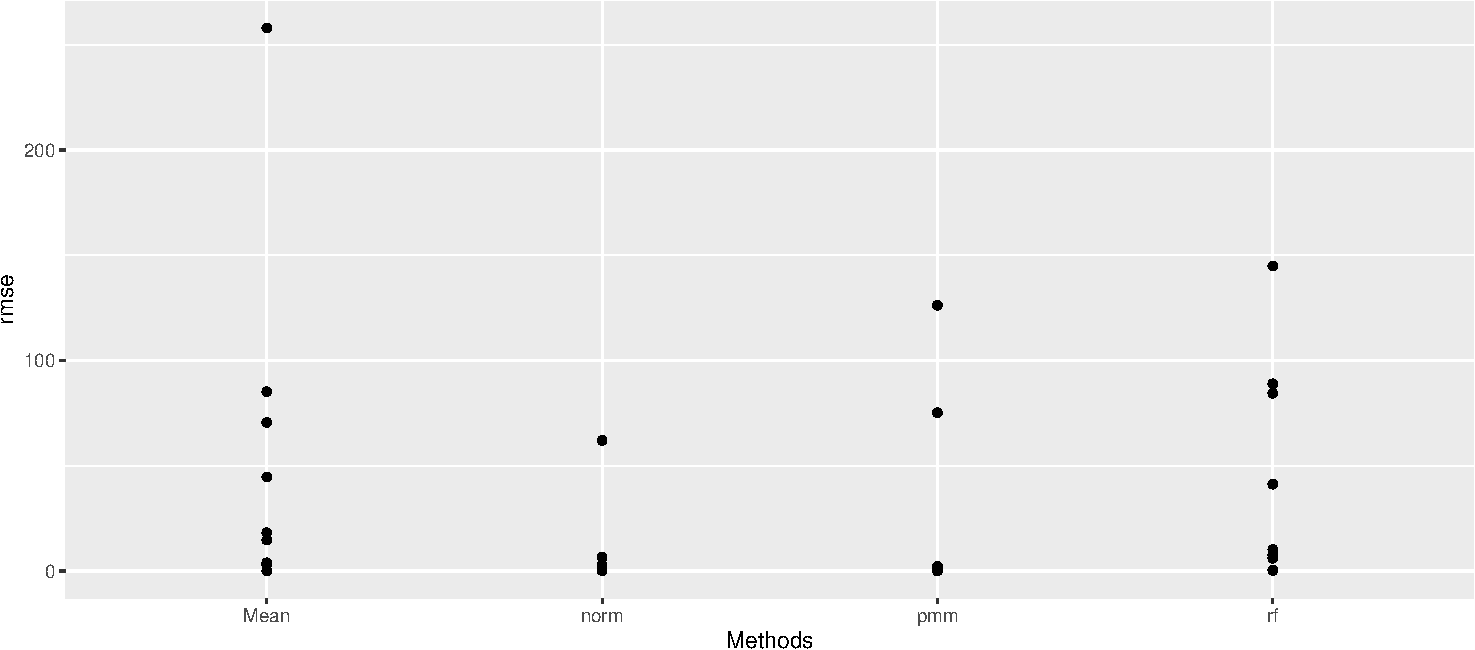
\includegraphics{repport_projet_files/figure-latex/unnamed-chunk-24-1.pdf}

En faisant une comparaison des quatre méthodologies d'imputations, nous
remarquons que les méthodes \textbf{norm} et \textbf{pmm} minimisent au
mieux les variables. Mais pour en choisir qu'une à la fin nous allons
vérifier les statistiques descriptives des données avant et après
imputation et surtout pour la variable RMSSD en phase T1 qui servira
plus tard pour la prédiction.

\hypertarget{comparaison-des-statistiques-descriptives-des-muxe9thodes-et-de-quelques-variables-pour-les-muxe9thodes-norm-et-pmm}{%
\subsubsection{Comparaison des statistiques descriptives des méthodes et
de quelques variables pour les méthodes norm et
pmm}\label{comparaison-des-statistiques-descriptives-des-muxe9thodes-et-de-quelques-variables-pour-les-muxe9thodes-norm-et-pmm}}

\hypertarget{donnuxe9es-originales}{%
\paragraph{Données originales:}\label{donnuxe9es-originales}}

\begin{table}[H]
\centering
\begin{tabular}{l|l|l|l|l|l}
\hline
  & T0\_Mean\_RR\_ms &  T0\_STD\_RR\_ms & T0\_Mean\_HR\_1\_min & T0\_STD\_HR\_1\_min &  T0\_RMSSD\_ms\\
\hline
 & Min.   : 654.9 & Min.   :  7.107 & Min.   :50.01 & Min.   :0.4276 & Min.   :  4.853\\
\hline
 & 1st Qu.: 827.8 & 1st Qu.: 25.279 & 1st Qu.:60.42 & 1st Qu.:1.8964 & 1st Qu.: 17.550\\
\hline
 & Median : 908.1 & Median : 35.295 & Median :66.84 & Median :2.4959 & Median : 26.012\\
\hline
 & Mean   : 914.6 & Mean   : 38.304 & Mean   :66.93 & Mean   :2.9802 & Mean   : 34.630\\
\hline
 & 3rd Qu.: 997.4 & 3rd Qu.: 45.589 & 3rd Qu.:72.59 & 3rd Qu.:3.4310 & 3rd Qu.: 40.421\\
\hline
 & Max.   :1200.8 & Max.   :122.626 & Max.   :91.79 & Max.   :9.4619 & Max.   :174.752\\
\hline
\end{tabular}
\end{table}

\hypertarget{donnuxe9es-imputuxe9es-par-norm}{%
\paragraph{Données imputées par
norm}\label{donnuxe9es-imputuxe9es-par-norm}}

\begin{table}[H]
\centering
\begin{tabular}{l|l|l|l|l|l}
\hline
  & T0\_Mean\_RR\_ms &  T0\_STD\_RR\_ms & T0\_Mean\_HR\_1\_min & T0\_STD\_HR\_1\_min &  T0\_RMSSD\_ms\\
\hline
 & Min.   : 654.9 & Min.   :  7.107 & Min.   :50.01 & Min.   :0.4276 & Min.   : -9.546\\
\hline
 & 1st Qu.: 827.8 & 1st Qu.: 25.387 & 1st Qu.:60.42 & 1st Qu.:1.9783 & 1st Qu.: 16.861\\
\hline
 & Median : 912.4 & Median : 35.308 & Median :66.85 & Median :2.4959 & Median : 24.875\\
\hline
 & Mean   : 914.9 & Mean   : 38.643 & Mean   :66.93 & Mean   :3.0289 & Mean   : 34.136\\
\hline
 & 3rd Qu.: 997.4 & 3rd Qu.: 47.137 & 3rd Qu.:72.59 & 3rd Qu.:3.4342 & 3rd Qu.: 38.238\\
\hline
 & Max.   :1200.8 & Max.   :122.626 & Max.   :91.79 & Max.   :9.4619 & Max.   :174.752\\
\hline
\end{tabular}
\end{table}

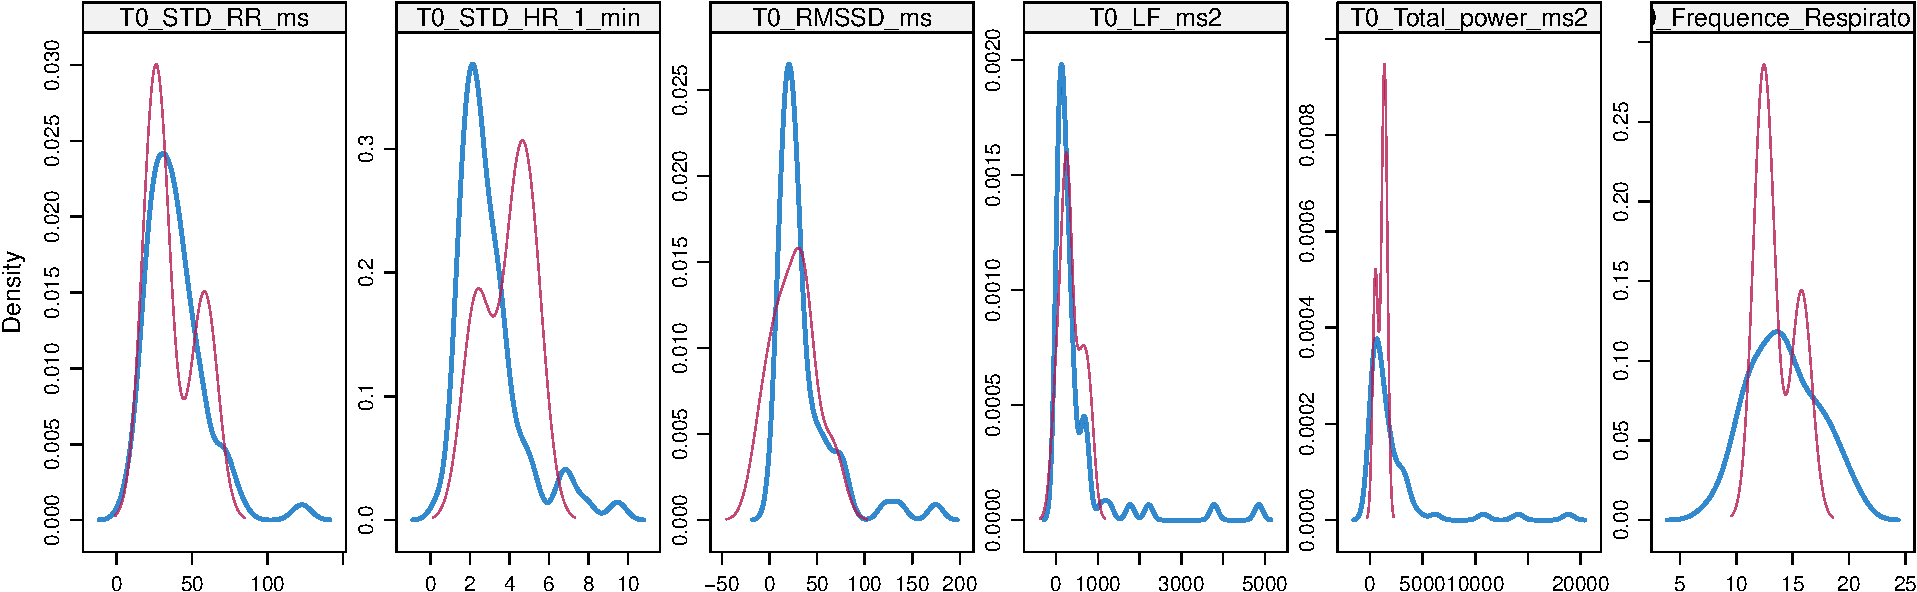
\includegraphics{repport_projet_files/figure-latex/unnamed-chunk-27-1.pdf}

En bleu la densité réelle, en rouge la densité après imputation.

Nous pouvons observer que la méthode norm renvoie une répartition
similaire à la répartition d'origine pour la variable LF et
potentiellement STD. Pour les autres variables ce n'est pas le cas, même
si on observe bien des moyennes très proche.

\hypertarget{donnuxe9es-imputuxe9es-par-pmm}{%
\paragraph{Données imputées par
pmm}\label{donnuxe9es-imputuxe9es-par-pmm}}

\begin{table}[H]
\centering
\begin{tabular}{l|l|l|l|l|l}
\hline
  & T0\_Mean\_RR\_ms &  T0\_STD\_RR\_ms & T0\_Mean\_HR\_1\_min & T0\_STD\_HR\_1\_min &  T0\_RMSSD\_ms\\
\hline
 & Min.   : 654.9 & Min.   :  7.107 & Min.   :50.01 & Min.   :0.4276 & Min.   :  4.853\\
\hline
 & 1st Qu.: 827.8 & 1st Qu.: 25.524 & 1st Qu.:60.42 & 1st Qu.:1.8964 & 1st Qu.: 17.084\\
\hline
 & Median : 908.1 & Median : 35.308 & Median :66.57 & Median :2.4959 & Median : 25.737\\
\hline
 & Mean   : 914.5 & Mean   : 38.420 & Mean   :66.92 & Mean   :2.9739 & Mean   : 35.022\\
\hline
 & 3rd Qu.: 997.4 & 3rd Qu.: 45.589 & 3rd Qu.:72.59 & 3rd Qu.:3.4251 & 3rd Qu.: 42.498\\
\hline
 & Max.   :1200.8 & Max.   :122.626 & Max.   :91.79 & Max.   :9.4619 & Max.   :174.752\\
\hline
\end{tabular}
\end{table}

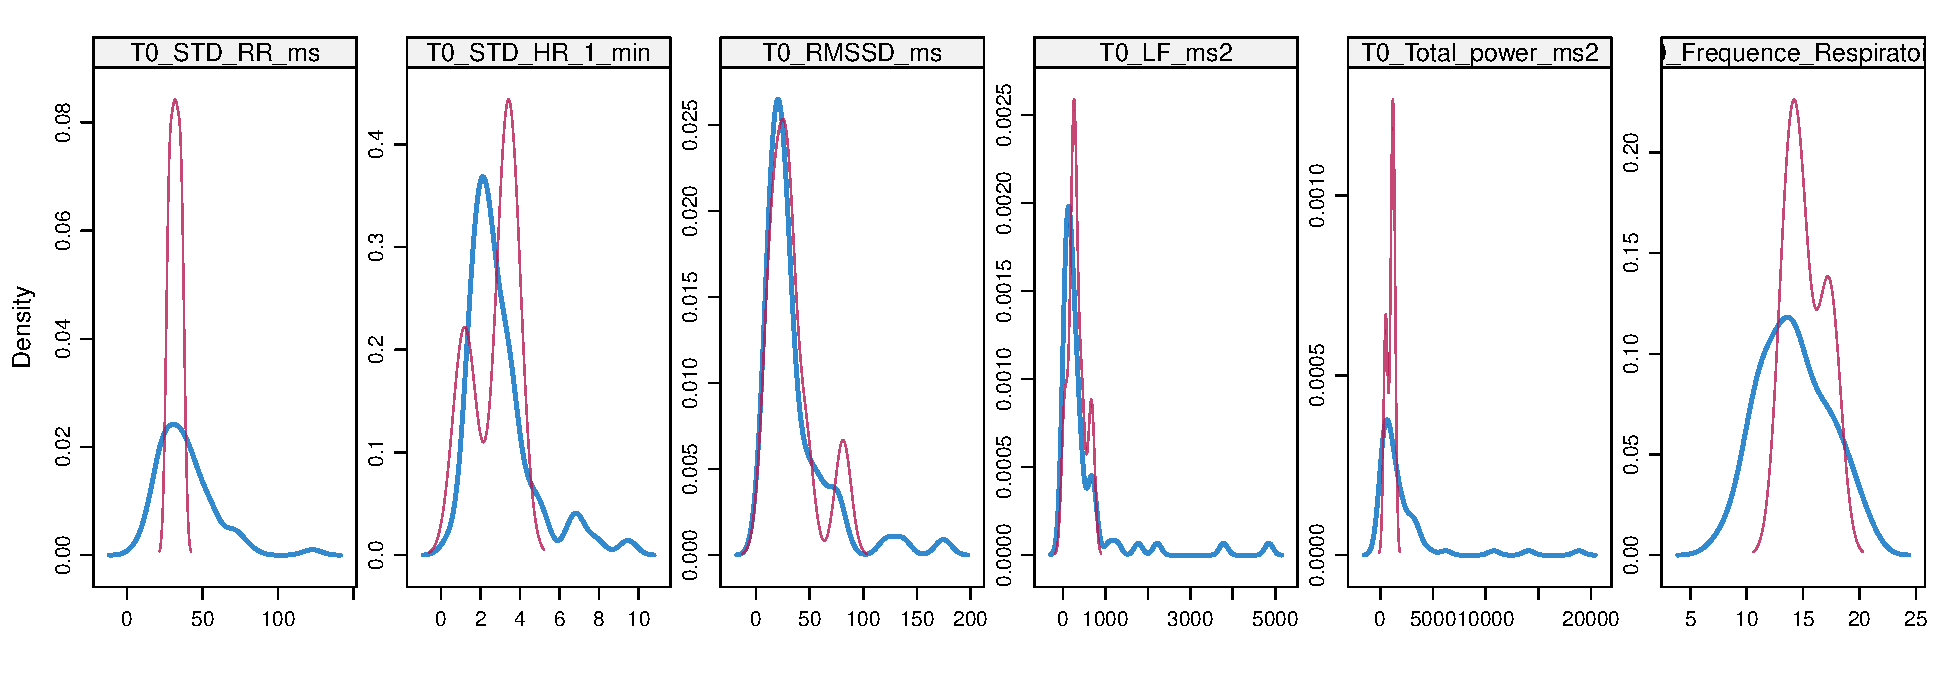
\includegraphics{repport_projet_files/figure-latex/unnamed-chunk-29-1.pdf}

En bleu la densité réelle, en rouge la densité après imputation.

Nous pouvons observer que la méthode renvoie une bonne répartition pour
les variable RMSSD et LF mais ce n'est pas autant le cas avec les autres
variables.

En regardant les statistiques descriptives, nous remarquons que les
valeurs de la méthode pmm se rapproche plus des vraies valeurs. D'autant
plus que la méthode Norm nous a donné des valeurs négatives. Nous allons
donc utiliser le pmm pour notre imputation.

\newpage

\hypertarget{imputation-uxe0-t1}{%
\subsection{Imputation à T1}\label{imputation-uxe0-t1}}

\begin{table}[H]
\centering
\begin{tabular}{r|r|r|r}
\hline
T1\_Mean\_RR\_ms & T1\_STD\_RR\_ms & T1\_Mean\_HR\_1\_min & T1\_STD\_HR\_1\_min\\
\hline
976.8550 & 50.7064 & 61.5833 & 3.1299\\
\hline
973.7792 & 62.8008 & 61.9898 & 6.3224\\
\hline
1238.2258 & 18.7991 & 48.4687 & 0.8212\\
\hline
1016.0228 & 35.9671 & 59.1288 & 2.1256\\
\hline
895.1647 & 31.4268 & 67.1114 & 2.4192\\
\hline
795.9072 & 22.4034 & 75.4457 & 2.1376\\
\hline
\end{tabular}
\end{table}

A T1, nous avons environ 57 observations et 10 variables avec 22 valeurs
manquantes.

\hypertarget{ruxe9partition-des-na-par-variables-1}{%
\subsubsection{Répartition des NA par
variables}\label{ruxe9partition-des-na-par-variables-1}}

Regardons le taux de valeurs manquantes pour chaque variable à T1:

\begin{table}[H]
\centering
\begin{tabular}{l|r}
\hline
  & \% NA\\
\hline
T0\_Mean\_RR\_ms & 2.47\\
\hline
T0\_STD\_RR\_ms & 7.41\\
\hline
T0\_Mean\_HR\_1\_min & 4.94\\
\hline
T0\_STD\_HR\_1\_min & 4.94\\
\hline
T0\_RMSSD\_ms & 7.41\\
\hline
T0\_VLF\_ms2 & 1.23\\
\hline
T0\_LF\_ms2 & 2.47\\
\hline
T0\_HF\_ms2 & 4.94\\
\hline
T0\_Total\_power\_ms2 & 4.94\\
\hline
T0\_Frequence\_Respiratoire & 2.47\\
\hline
\end{tabular}
\end{table}

Vu la taille de nos données, nous pouvons dire que les taux de valeurs
manquantes ne sont pas négligeables.

\hypertarget{comparaison-des-ruxe9sultats}{%
\subsubsection{Comparaison des
résultats}\label{comparaison-des-ruxe9sultats}}

Considérons notre tableau de données sans les NA, puis créons
artificiellement et aléatoirement 5\% de valeurs manquantes. Nous
obtenons ces résultats:

\begin{table}[H]
\centering
\begin{tabular}{l|r|r|r|r|r}
\hline
  & mean & pmm & rf & norm & BestRmse\\
\hline
T1\_Mean\_RR\_ms & 13.63 & 13.63 & 15.10 & 5.48 & 5.48\\
\hline
T1\_STD\_RR\_ms & 0.03 & 0.03 & 0.83 & 0.50 & 0.03\\
\hline
T1\_Mean\_HR\_1\_min & 0.82 & 0.82 & 3.09 & 0.74 & 0.74\\
\hline
T1\_STD\_HR\_1\_min & 0.10 & 0.10 & 0.25 & 0.19 & 0.10\\
\hline
T1\_RMSSD\_ms & 0.30 & 0.30 & 3.27 & 3.90 & 0.30\\
\hline
T1\_VLF\_ms2 & 33.21 & 33.21 & 40.91 & 79.80 & 33.21\\
\hline
T1\_LF\_ms2 & 355.80 & 355.80 & 303.44 & 7.15 & 7.15\\
\hline
T1\_HF\_ms2 & 970.33 & 970.33 & 952.02 & 753.12 & 753.12\\
\hline
T1\_Total\_power\_ms2 & 1096.94 & 1096.94 & 478.19 & 758.99 & 478.19\\
\hline
T1\_Frequence\_Respiratoire & 1.08 & 1.08 & 0.18 & 0.63 & 0.18\\
\hline
\end{tabular}
\end{table}

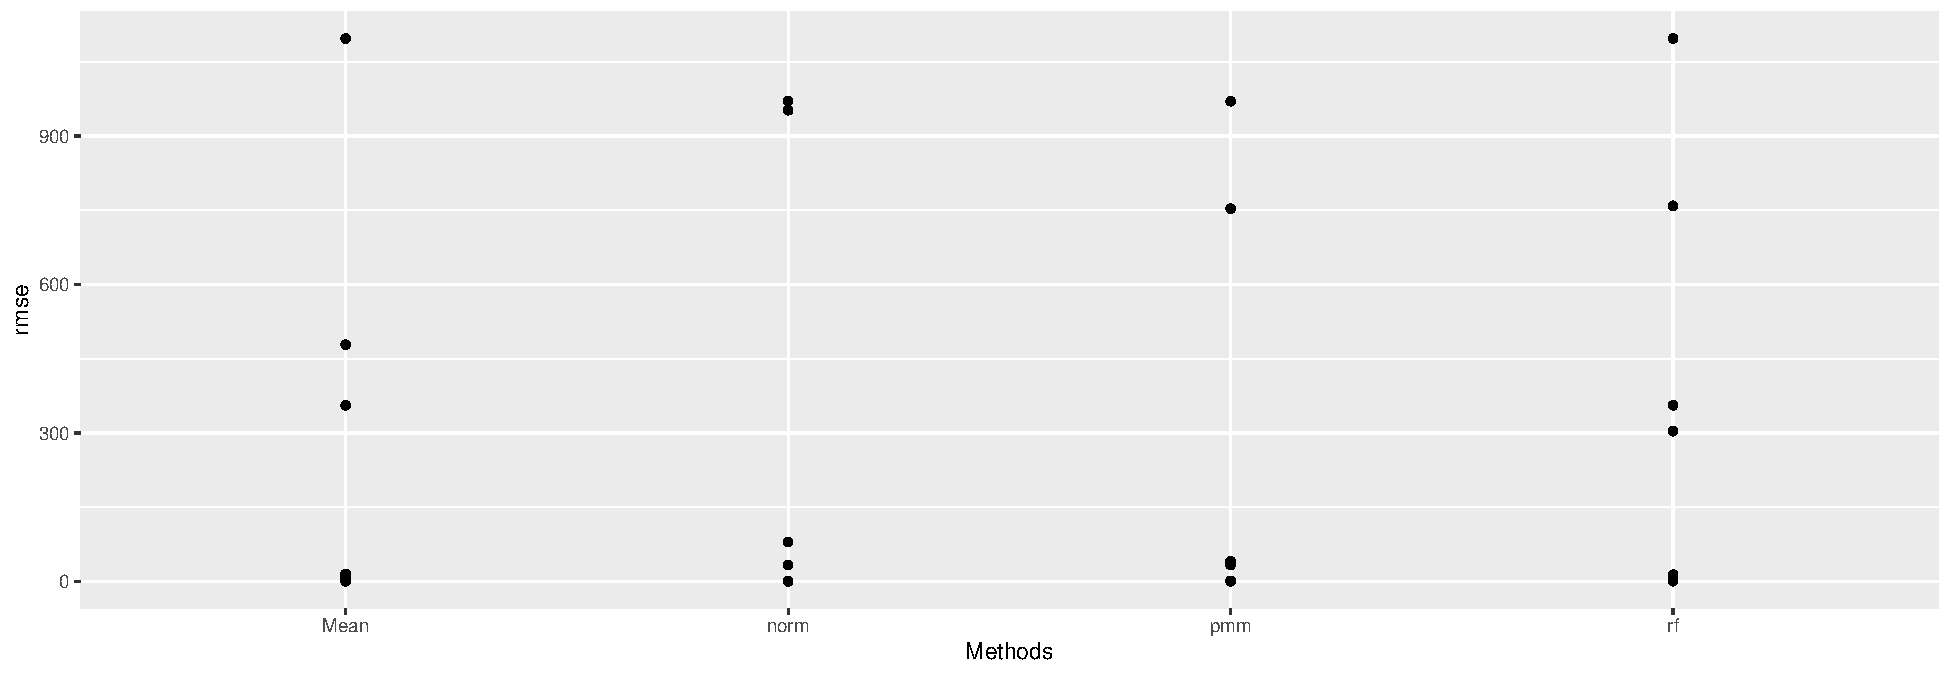
\includegraphics{repport_projet_files/figure-latex/unnamed-chunk-36-1.pdf}

Nous remarquons que les méthodes \textbf{norm} et \textbf{pmm} ont les
RMSE les plus faibles et donnent donc de meilleurs résultats. Mais pour
en choisir qu'une à la fin nous allons voir les statistiques
descriptives des données avant et après imputation et surtout pour la
variable RMSSD en phase T1 qui servira plus tard pour la prédiction.

\hypertarget{comparaison-des-statistiques-descriptives-de-quelques-variables-pour-les-muxe9thodes-norm-et-pmm}{%
\subsubsection{Comparaison des statistiques descriptives de quelques
variables pour les méthodes norm et
pmm}\label{comparaison-des-statistiques-descriptives-de-quelques-variables-pour-les-muxe9thodes-norm-et-pmm}}

\hypertarget{donnuxe9es-originales-1}{%
\paragraph{Données originales:}\label{donnuxe9es-originales-1}}

\begin{table}[H]
\centering
\begin{tabular}{l|l|l|l|l|l}
\hline
  & T1\_Mean\_RR\_ms &  T1\_STD\_RR\_ms & T1\_Mean\_HR\_1\_min & T1\_STD\_HR\_1\_min &  T1\_RMSSD\_ms\\
\hline
 & Min.   : 598.9 & Min.   :  7.107 & Min.   : 48.47 & Min.   : 0.4276 & Min.   :  4.618\\
\hline
 & 1st Qu.: 827.8 & 1st Qu.: 26.849 & 1st Qu.: 58.97 & 1st Qu.: 1.8960 & 1st Qu.: 14.343\\
\hline
 & Median : 952.0 & Median : 35.540 & Median : 63.10 & Median : 2.2972 & Median : 25.749\\
\hline
 & Mean   : 937.1 & Mean   : 41.142 & Mean   : 65.84 & Mean   : 3.2437 & Mean   : 36.865\\
\hline
 & 3rd Qu.:1019.0 & 3rd Qu.: 50.265 & 3rd Qu.: 73.08 & 3rd Qu.: 3.2837 & 3rd Qu.: 36.300\\
\hline
 & Max.   :1238.2 & Max.   :120.334 & Max.   :100.24 & Max.   :12.6799 & Max.   :178.357\\
\hline
\end{tabular}
\end{table}

\hypertarget{donnuxe9es-imputuxe9es-par-norm-1}{%
\paragraph{Données imputées par
norm}\label{donnuxe9es-imputuxe9es-par-norm-1}}

\begin{table}[H]
\centering
\begin{tabular}{l|l|l|l|l|l}
\hline
  & T1\_Mean\_RR\_ms &  T1\_STD\_RR\_ms & T1\_Mean\_HR\_1\_min & T1\_STD\_HR\_1\_min &  T1\_RMSSD\_ms\\
\hline
 & Min.   : 598.9 & Min.   :  7.107 & Min.   : 48.47 & Min.   : 0.2095 & Min.   :-19.08\\
\hline
 & 1st Qu.: 827.8 & 1st Qu.: 26.849 & 1st Qu.: 59.05 & 1st Qu.: 1.8122 & 1st Qu.: 14.14\\
\hline
 & Median : 952.0 & Median : 35.540 & Median : 63.10 & Median : 2.2972 & Median : 25.75\\
\hline
 & Mean   : 937.4 & Mean   : 41.212 & Mean   : 65.90 & Mean   : 3.2070 & Mean   : 36.11\\
\hline
 & 3rd Qu.:1019.0 & 3rd Qu.: 50.265 & 3rd Qu.: 73.08 & 3rd Qu.: 3.2837 & 3rd Qu.: 36.30\\
\hline
 & Max.   :1238.2 & Max.   :120.334 & Max.   :100.24 & Max.   :12.6799 & Max.   :178.36\\
\hline
\end{tabular}
\end{table}

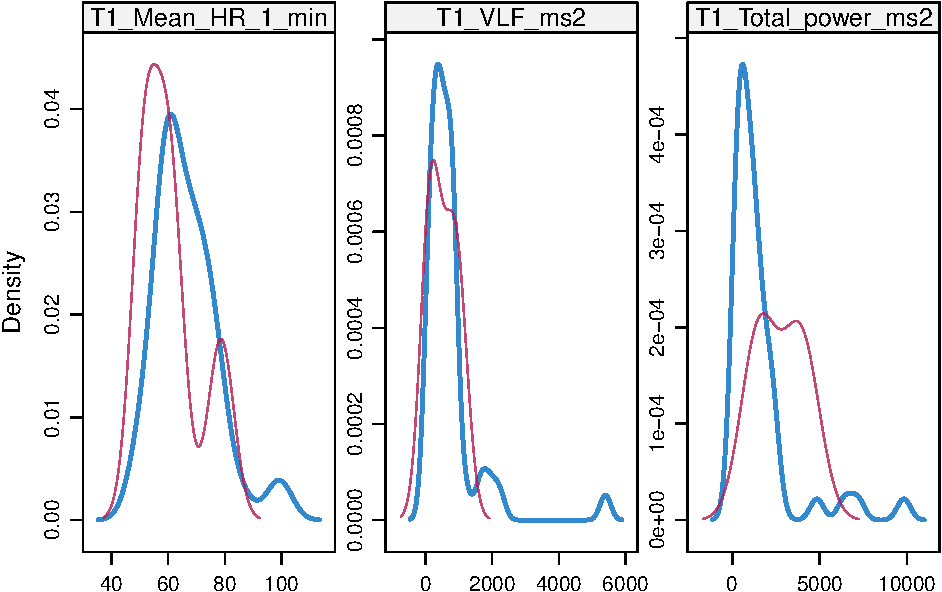
\includegraphics{repport_projet_files/figure-latex/unnamed-chunk-39-1.pdf}

En bleu la densité réelle, en rouge la densité après imputation.

Nous pouvons observer que la méthode norm renvoie une répartition assez
similaire à la répartition d'origine pour la variable MEAN HR et
potentiellement VLF. Pour les autres variables ce n'est pas le cas, même
si on observe bien des moyennes très proche.

\hypertarget{donnuxe9es-imputuxe9es-par-pmm-1}{%
\paragraph{Données imputées par
pmm}\label{donnuxe9es-imputuxe9es-par-pmm-1}}

\begin{table}[H]
\centering
\begin{tabular}{l|l|l|l|l|l}
\hline
  & T0\_Mean\_RR\_ms &  T0\_STD\_RR\_ms & T0\_Mean\_HR\_1\_min & T0\_STD\_HR\_1\_min &  T0\_RMSSD\_ms\\
\hline
 & Min.   : 654.9 & Min.   :  7.107 & Min.   :50.01 & Min.   :0.4276 & Min.   :  4.853\\
\hline
 & 1st Qu.: 827.8 & 1st Qu.: 25.524 & 1st Qu.:60.42 & 1st Qu.:1.8964 & 1st Qu.: 17.084\\
\hline
 & Median : 908.1 & Median : 35.308 & Median :66.57 & Median :2.4959 & Median : 25.737\\
\hline
 & Mean   : 914.5 & Mean   : 38.420 & Mean   :66.92 & Mean   :2.9739 & Mean   : 35.022\\
\hline
 & 3rd Qu.: 997.4 & 3rd Qu.: 45.589 & 3rd Qu.:72.59 & 3rd Qu.:3.4251 & 3rd Qu.: 42.498\\
\hline
 & Max.   :1200.8 & Max.   :122.626 & Max.   :91.79 & Max.   :9.4619 & Max.   :174.752\\
\hline
\end{tabular}
\end{table}

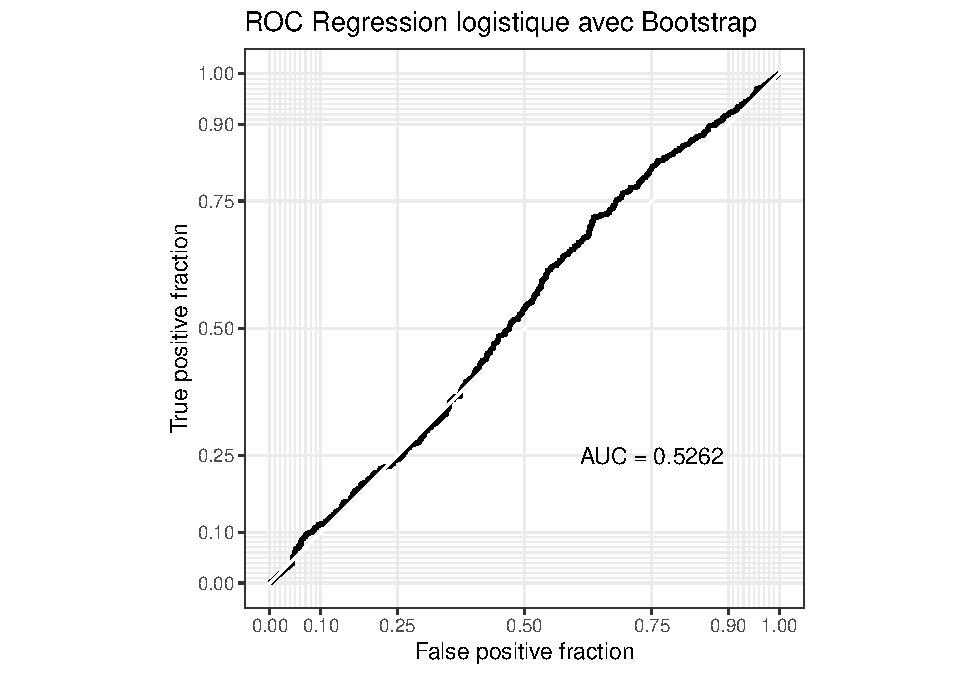
\includegraphics{repport_projet_files/figure-latex/unnamed-chunk-41-1.pdf}

En bleu la densité réelle, en rouge la densité après imputation.

Nous pouvons observer que la méthode renvoie une assez bonne répartition
pour des variables mais ce n'est pas autant le cas pour la variable MEAN
HR.

En regardant les statistiques descriptives, nous remarquons que les
valeurs de la méthode pmm se rapproche plus des vraies valeurs.
Globalement, les résultats sont très proche de la réalité et même si
parfois, l'estimation bayesienne donne de meilleur résultat, nous
pouvons observer que la méthode pmm est dans l'ensemble plus efficace.

\emph{Conclusion} : Notre jeu de données sera imputé par la méthode de
la moyenne prévisionnelle qui donne de meilleurs résultats en T0 et T1.

Pour la suite nous allons combiner nos données en T0 et T1 afin de créer
nos modèles, nous nous retrouvons donc avec 48 observations et 20
colonnes.

\hypertarget{comparaison-avant-et-apruxe8s-imputation}{%
\subsubsection{Comparaison avant et après
imputation}\label{comparaison-avant-et-apruxe8s-imputation}}

\emph{RMSSD Avant Imputation:}

\begin{table}[H]
\centering
\begin{tabular}{l|l|l}
\hline
  &  T0\_RMSSD\_ms &  T1\_RMSSD\_ms\\
\hline
 & Min.   :  4.853 & Min.   :  4.618\\
\hline
 & 1st Qu.: 20.021 & 1st Qu.: 14.851\\
\hline
 & Median : 28.035 & Median : 25.749\\
\hline
 & Mean   : 44.796 & Mean   : 39.956\\
\hline
 & 3rd Qu.: 57.952 & 3rd Qu.: 44.460\\
\hline
 & Max.   :214.604 & Max.   :178.357\\
\hline
 & NA's   :4 & NA's   :3\\
\hline
\end{tabular}
\end{table}

\emph{RMSSD Après Imputation:}

\begin{table}[H]
\centering
\begin{tabular}{l|l|l}
\hline
  &  T0\_RMSSD\_ms &  T1\_RMSSD\_ms\\
\hline
 & Min.   :  4.853 & Min.   :  4.618\\
\hline
 & 1st Qu.: 20.021 & 1st Qu.: 17.094\\
\hline
 & Median : 28.035 & Median : 28.166\\
\hline
 & Mean   : 44.678 & Mean   : 40.341\\
\hline
 & 3rd Qu.: 57.952 & 3rd Qu.: 51.035\\
\hline
 & Max.   :214.604 & Max.   :178.357\\
\hline
\end{tabular}
\end{table}

En observant par exemple pour la variable RMSSD avant imputation et
après imputation, nous obtenons une moyenne de 44.79 en T0 et 39.95 en
T1 contre 44.67 en T0 et 40.34 , les valeurs sont donc assez similaires.

\hypertarget{bootstrap-comparaison-de-moyennes}{%
\subsection{Bootstrap: comparaison de
moyennes}\label{bootstrap-comparaison-de-moyennes}}

Pour terminer nos analyses, nous souhaitons identifier de nouveau si il
y a eu une amélioration général de l'état de santé des patients. Nous
allons donc comparer les moyennes de notre échantillon. Au vu du faible
de nombre de données, afin de parfaire nos estimations de la moyenne,
nous avons utilisé la méthode du Bootstrap. Nous regardons surtout la
variable RMSSD qui est un bon indicaeur de cette amélioration. Nous
avons donc tiré 200 échantillons, et pour chacun d'eux, avons calculé
les moyennes en T0 et T1 et appliqué un Test de Wilcoxon sur ces
moyennes obtenues. Nous avons donc comme hypothèses:

\begin{itemize}
\tightlist
\item
  H0: T0\textgreater{}T1
\item
  H1: T0\textless{}T1
\end{itemize}

\begin{table}[H]
\centering
\begin{tabular}{r|r|r}
\hline
M0\_boot & M1\_boot & pval\_boot\\
\hline
44.40285 & 39.95523 & 0.2798285\\
\hline
\end{tabular}
\end{table}

Nous avons une p-value= 0.2798285 qui est supérieure à 0.05, donc on
conserve H0 au seuil de 5\%; il y a bien une amélioration.

\hypertarget{construction-de-moduxe8les}{%
\section{Construction de modèles}\label{construction-de-moduxe8les}}

Maintenant que nous avons imputé nos variables, nous pouvons chercher à
créer un modèle pour prédire si une personne a vu sa condition physique
s'améliorer. Pour cela, nous n'utilisons que les variables du temps T0.

Avec moins d'une cinquantaine d'individus dans nos résultats finaux,
nous décidons de simplement chercher un modèle avec l'ensemble de nos
données. Il faudra alors espérer avoir plus d'individus dans le futur
afin de tester nos modèles.

\hypertarget{optimisation-via-leave-one-out}{%
\subsection{Optimisation via Leave one
Out}\label{optimisation-via-leave-one-out}}

Nous allons chercher ici à optimiser nos modèles via la validation
croisée. La méthode de validation croisée Leave one out permet de faire
des tests avec peu d'individus.

\hypertarget{regression-logistique-1}{%
\subsubsection{Regression logistique}\label{regression-logistique-1}}

La première méthode que nous allons utiliser ici est la regression
logistique descendante.

La précision de notre modèle est d'environ 0.5208333, ce qui est
légèrement meilleur qu'un modèle renvoyant toujours la même prédiction
avec nos données. Les variables conservée sont les variables RMSSD, VLF,
HF, Mean HR, STD RR. Les variables conservées sont principalement celles
que l'on considère souvent comme assez importantes dans la litterature
scientifique. Parmis ce type de variable, seul LF a été écartée.

\hypertarget{svm-1}{%
\subsubsection{SVM}\label{svm-1}}

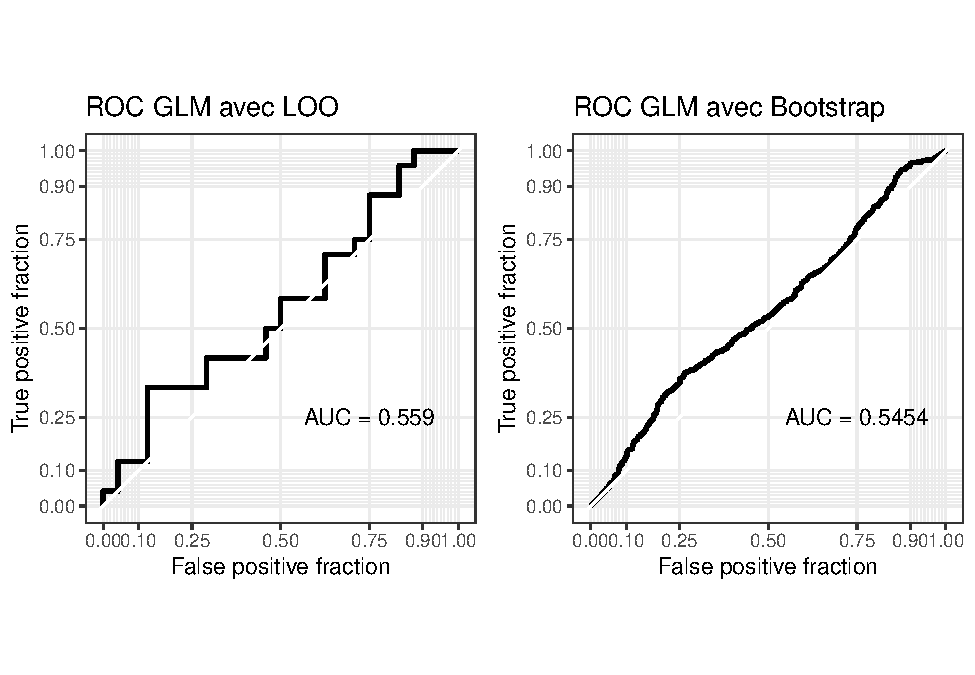
\includegraphics{repport_projet_files/figure-latex/unnamed-chunk-51-1.pdf}

Le SVM ici a dans l'ensemble un accuracy proche ou inférieur à 50\%. Vu
nos données, cela signifie qu'il est moins bon qu'un predicteur
prédisant toujours la même valeur.

\hypertarget{randomforest}{%
\subsubsection{randomForest}\label{randomforest}}

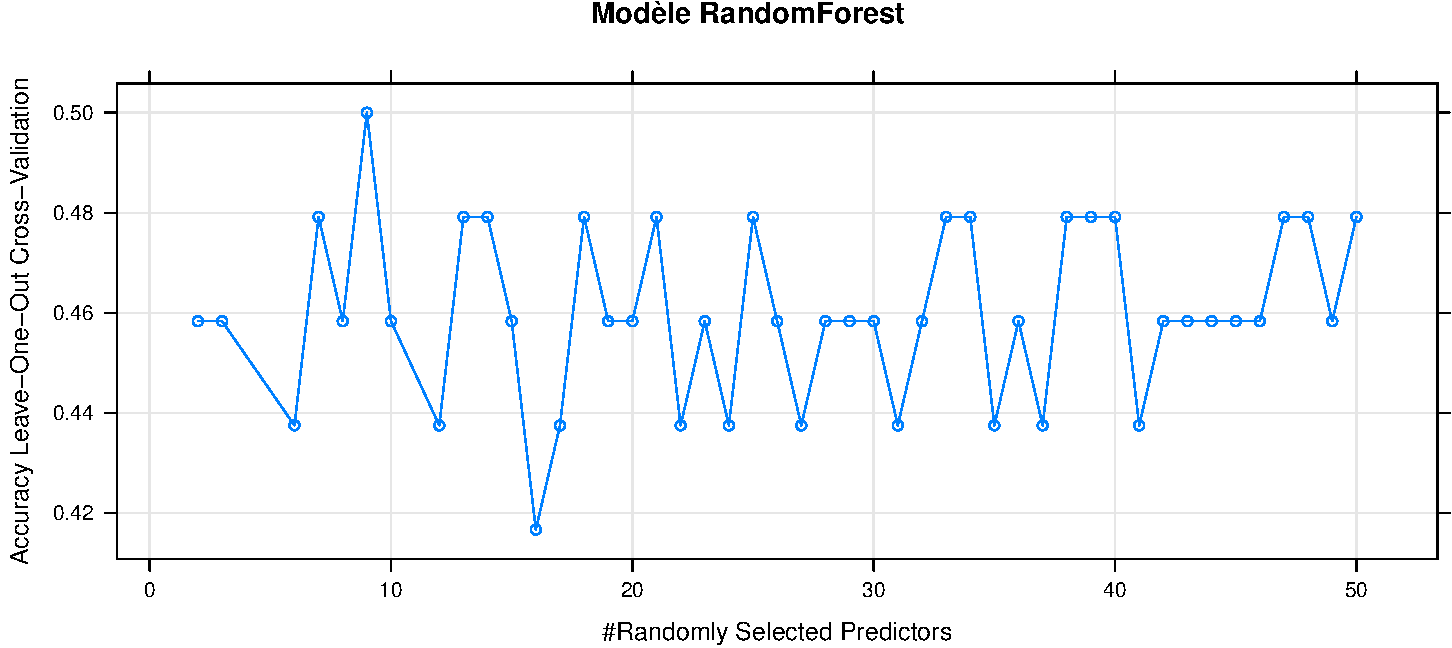
\includegraphics{repport_projet_files/figure-latex/unnamed-chunk-52-1.pdf}

Optimiser la méthode de forêt aléatoire avec la validation croisée
``Leave One Out'' n'est pas évidente. En effet, l'évaluation via un seul
individu ne permet pas d'obtenir de résultat robuste dans ce cas là car
le résultat dépend trop des variables choisies. De plus, l'accuracy,
qu'importe le nombre de variable, semble se stabiliser vers 50\% ou
moins, ce qui est actuellement moins efficace qu'un predicteur prédisant
toujours la même variable dans notre cas.

\hypertarget{optimisation-via-bootstrap}{%
\subsection{Optimisation via
Bootstrap}\label{optimisation-via-bootstrap}}

Ici, nous allons utiliser une autre méthode, le bootstrap pour essayer
de contourner notre problème de manque de donnée.

\hypertarget{regression-logistique-2}{%
\subsubsection{Regression logistique}\label{regression-logistique-2}}

La précision de notre modèle est d'environ 0.5176385, ce qui est
légèrement meilleur qu'un modèle renvoyant toujours la même prédiction
avec nos données. Les variables conservée sont les variables RMSSD, VLF,
HF, Mean HR, STD RR. Les variables conservées sont principalement celles
que l'on considère souvent comme assez importantes dans la litterature
scientifique. Parmis ce type de variable, seul LF a été écartée.

Au final, on retrouve pratiquement le même résultat qu'avec le leave one
out.

\hypertarget{svm-2}{%
\subsubsection{SVM}\label{svm-2}}

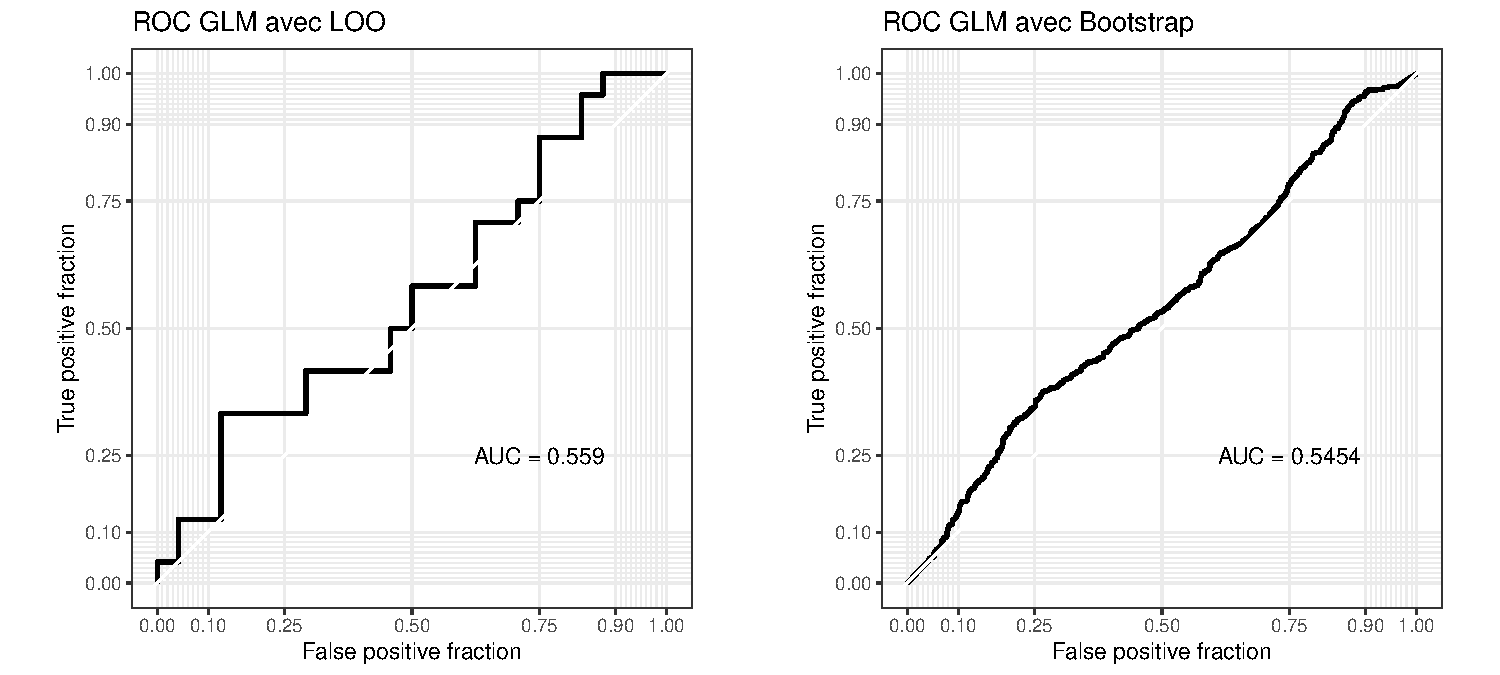
\includegraphics{repport_projet_files/figure-latex/unnamed-chunk-55-1.pdf}

Le SVM ici a dans l'ensemble un accuracy proche ou inférieur à 50\%. Vu
nos données, cela signifie qu'il est moins bon qu'un predicteur
prédisant toujours la même valeur.

\hypertarget{randomforest-1}{%
\subsubsection{randomForest}\label{randomforest-1}}

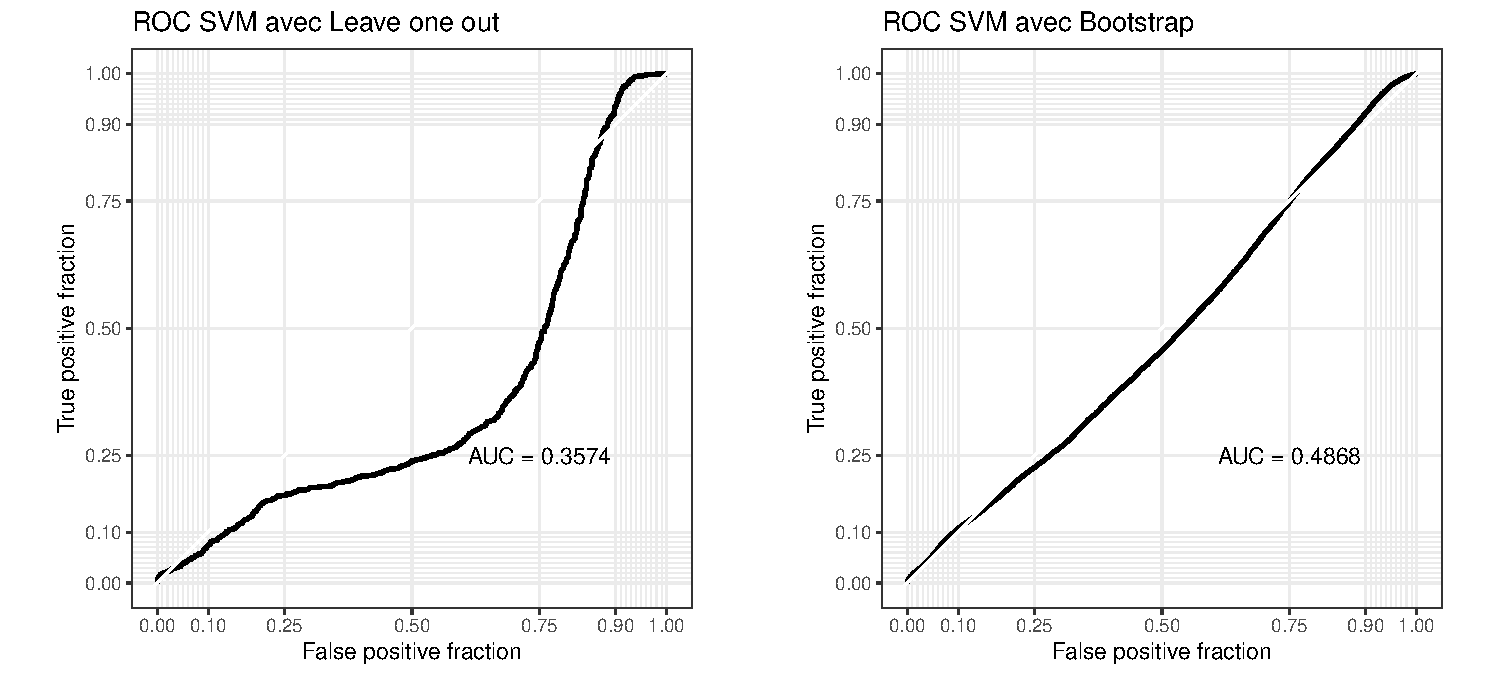
\includegraphics{repport_projet_files/figure-latex/unnamed-chunk-56-1.pdf}

L'accuracy, qu'importe le nombre de variable, semble se stabiliser vers
50\% ou moins, ce qui est actuellement moins efficace qu'un predicteur
prédisant toujours la même variable dans notre cas.

\hypertarget{comparaisons}{%
\subsection{Comparaisons}\label{comparaisons}}

Nous avons vu que quelques soit les méthodes d'évaluation et de
prédiction que nous utilisons, dans l'ensemble, nous obtenons souvent
des résultats semblables, avec une précision proche de 50\%. Nous allons
maintenant terminer en comparant nos méthodes selon d'autres critères
afin d'arrêter notre choix. Pour cela, nous regardons les courbes ROC.

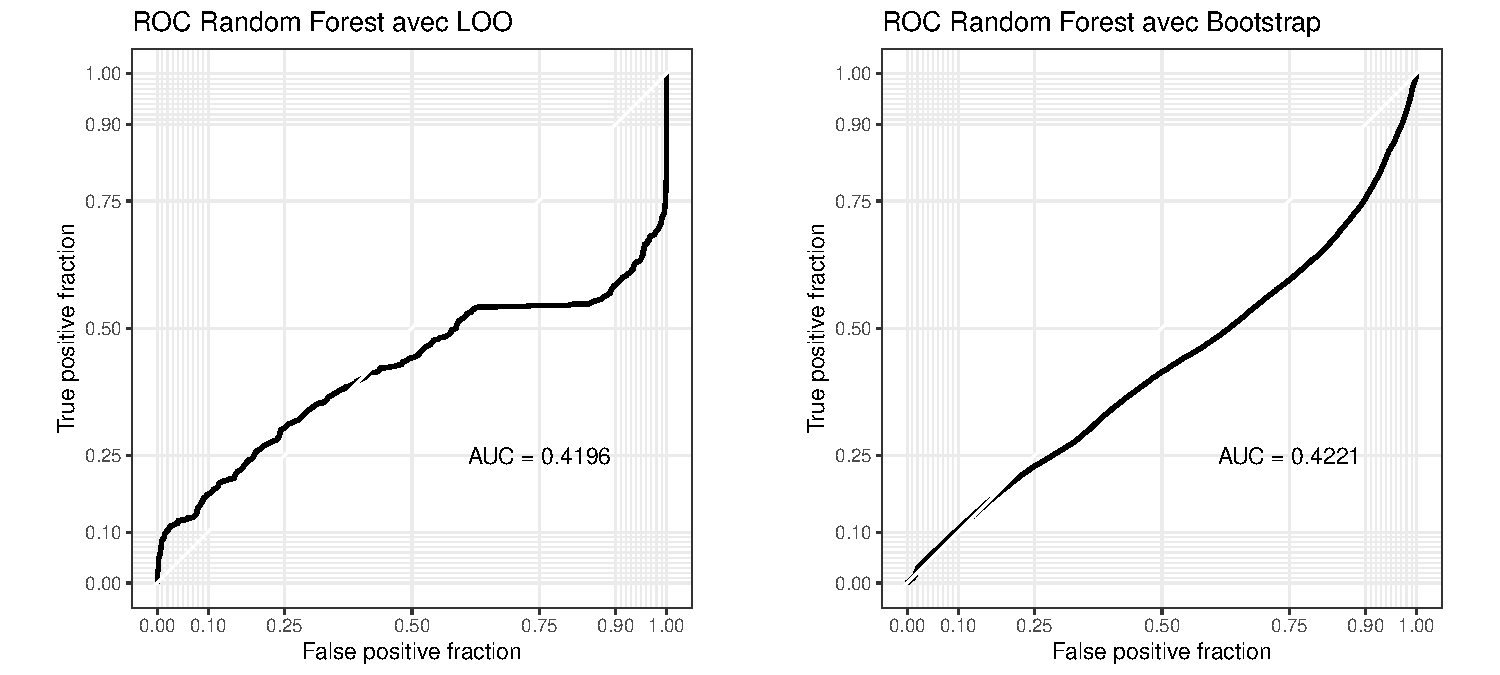
\includegraphics{repport_projet_files/figure-latex/unnamed-chunk-57-1.pdf}

Dans l'ensemble, on peut supposer que l'AUC de la regression logistique
est d'environ 0.55 .

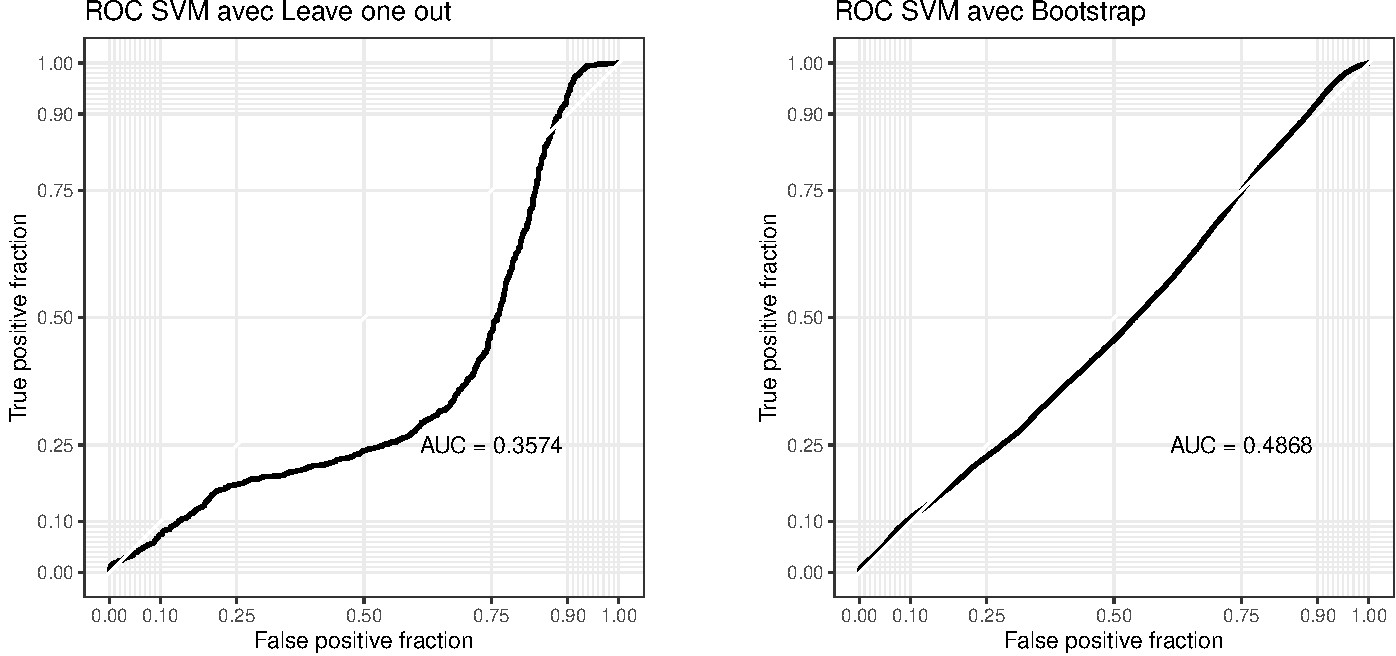
\includegraphics{repport_projet_files/figure-latex/unnamed-chunk-58-1.pdf}

Dans l'ensemble, on peut supposer que l'AUC du SVM est d'environ 0.48 .
C'est moins qu'avec la regression logistique.

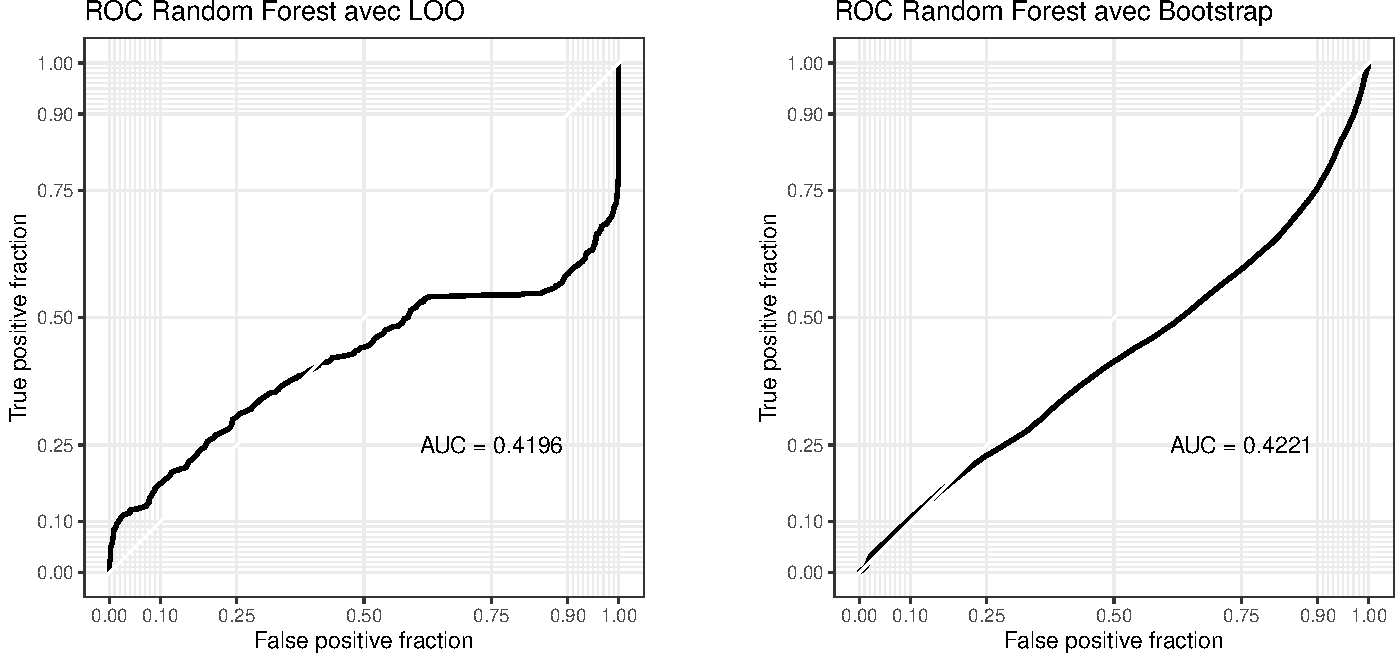
\includegraphics{repport_projet_files/figure-latex/unnamed-chunk-59-1.pdf}

Dans l'ensemble, on peut supposer que l'AUC du random Forest est
d'environ 0.43, c'est encore inférieur au SVM et à la regression
logistique.

\hypertarget{conclusion}{%
\section{Conclusion}\label{conclusion}}

Concernant l'imputation, nous avons pu voir que plusieurs méthodes
etaient possibles. La taille de nos données ne fut pas spécialement
contraignante et nons avons pu renvoyer des résultats satisfaisants. En
sachant que les relevés physiologiques sont souvent soumis à des erreurs
quand ils concernent des personnes après des problèmes cardiaques, nous
pouvons aisement imaginer que l'imputation permettra de compenser cela
dans des expériences futures.

Concernant les modèles de prédictions, nous pouvons voir qu'avec nos
données, il semble difficile d'établir un modèle convenable. Même si
nous utilisons différentes méthodes pour la recherche de predicteur
efficace, nous avons au final une précision faible dans tout les cas. Il
semble alors pour le moment difficile de prédire l'amélioration de
l'état de santé d'un individus via le programme en se basant seulement
sur des informations physilogiques avant expérience.

Enfin, pour conclure, il est à noter qu'il est possible que la méthode
du RandomForest puisse renvoyer de meilleures prédictions. En effet, il
suffirait d'inverser le modèle et nous aurions alors un modèle de
prédiction avec une précision plus grande. Ainsi, on peut imaginer
qu'avec beaucoup plus de données et surement d'itération, il est
possible de voir apparaître un modèle acceptable.


\end{document}
